\documentclass{article}
\usepackage[utf8]{inputenc}
\usepackage{tikz} 
\usepackage{float}
\usepackage{adjustbox}
\usepackage[left=1in, right=1in, top=1in, bottom=1in]{geometry}

\title{Tikz}
\author{}
\date{} 
 
\begin{document}
\maketitle
\begin{figure}[H]
\centering
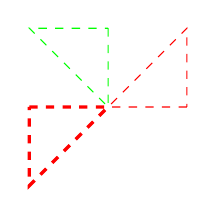
\begin{tikzpicture}
\draw[red, dashed] (1,0) -- (0,0) -- (1,1) -- cycle;
\draw[green, dashed, rotate=90] (1,0) -- (0,0) -- (1,1) -- cycle;
\draw[red, dashed, rotate=180, very thick] (1,0) -- (0,0) -- (1,1) -- cycle;
\end{tikzpicture} 
\caption{Unir puntos, cerrar figuras(cycle), color y  rotar}
\end{figure}

Uso del paquete adjustbox. Uso de perpendiculares y curvaturas
\begin{figure}[H]
\centering
\begin{adjustbox} {width=0.4\textwidth}
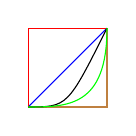
\begin{tikzpicture}
\draw[blue] (0,0) -- (1,1);
\draw[red] (0,0) |- (1,1);
\draw[brown] (0,0) -| (1,1);
\draw[black] (0,0) ..controls(0.5,0) .. (1,1);
\draw[green] (0,0) ..controls(0.5,0) and (1,0) .. (1,1);
\end{tikzpicture} 
\end{adjustbox}
\caption{Uso del paquete adjustbox. Uso de perpendiculares y curvaturas}
\end{figure}



\begin{figure}[H]
\centering
\begin{adjustbox} {width=0.4\textwidth}
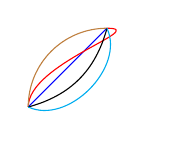
\begin{tikzpicture}
\draw[blue] (0,0) to (1,1);
\draw[red] (0,0) to[out=90, in=0] (1,1);
\draw[brown] (0,0) to[out=90, in=180] (1,1);
\draw[black] (0,0) to[bend right=30] (1,1);
\draw[cyan] (0,0) to[bend right=70] (1,1);
\end{tikzpicture} 
\end{adjustbox}
\caption{manera alterna con to, out para el punto de salida e in para el punto de entrada. Uso de bend right o bend left para curvaturas}
\end{figure}



\begin{figure}[H]
\centering
\begin{adjustbox} {width=0.4\textwidth}
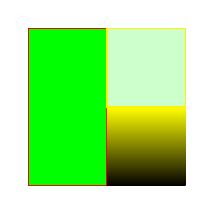
\begin{tikzpicture}
\draw[red,fill=green] (0,0) rectangle (1,2);
\shade[top color=yellow, bottom color=black] (1,0) rectangle (2,1);
\filldraw[fill=green!20!white, draw=yellow] (1,1) rectangle (2,2);
\end{tikzpicture} 
\end{adjustbox}
\caption{dibujar rectangulo con llenado y rectangulo degradado. Usp de filldraw}
\end{figure}



\begin{figure}[H]
\centering
\begin{adjustbox} {width=0.4\textwidth}
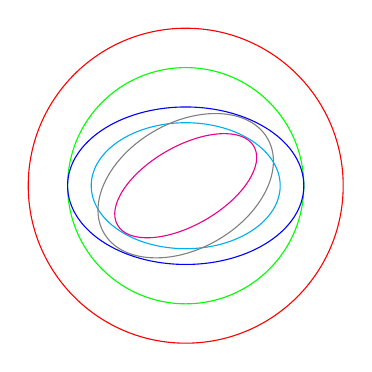
\begin{tikzpicture}
\draw[red] (0,0) circle (2cm);
\draw[green] (0,0) circle [radius=1.5cm];
\draw[cyan] (0,0) circle (1.2cm and 8mm);
\draw[gray, rotate=30] (0,0) circle (1.2cm and 8mm);
\draw[blue] (0,0) circle [x radius=1.5cm, y radius=10mm];
\draw[magenta] (0,0) circle [x radius=1cm, y radius=5mm, rotate=30];
\end{tikzpicture}
\end{adjustbox}
\caption{dibujando circulos y elipsis}
\end{figure}

\begin{figure}[H]
\centering
\begin{adjustbox} {width=0.4\textwidth}
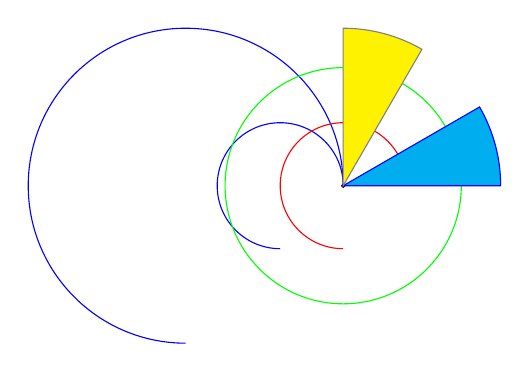
\begin{tikzpicture}
\draw[blue] (0,0) arc (0:270:2cm);
\draw[blue] (0,0) arc (0:270:8mm);
\draw[fill=black] (0,0) circle (0.2mm);
\draw[green] (0,0) circle (1.5);
\draw[red, shift={(8mm,0)}] (0,0) arc (0:270:8mm);
\filldraw[fill=cyan, draw=blue] (0,0) -- (2,0) arc (0:30:2) -- cycle;
\filldraw[fill=yellow, draw=gray, rotate=60] (0,0) -- (2,0) arc (0:30:2) -- cycle;
\end{tikzpicture}
\end{adjustbox}
\caption{sectores circulares, traslados con shift}
\end{figure}


\begin{figure}[H]
\centering
\begin{adjustbox} {width=0.4\textwidth}
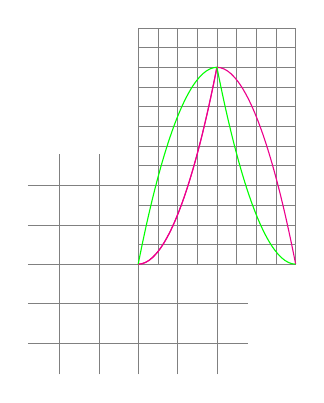
\begin{tikzpicture}
\draw[help lines, step=0.25] (0,0) grid (2,3);
\draw[gray, step=0.5, very thin] (-1.4,-1.4) grid (1.4,1.4);
\draw[magenta] (0,0) parabola (1,2.5);
\draw[magenta] (0,0) parabola (1,2.5) parabola (2,0);
\draw[green] (0,0) parabola[bend at end] (1,2.5) parabola[bend at end] (2,0);
\end{tikzpicture}
\end{adjustbox}
\caption{uso de cuadricula con grid, uso de parabola y concavidad,}
\end{figure}


\begin{figure}[H]
\centering
\begin{adjustbox} {width=0.4\textwidth}
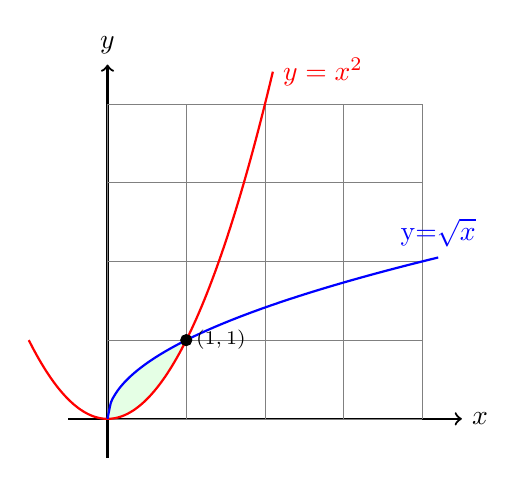
\begin{tikzpicture}
\draw[thick,->] (-0.5,0)--(4.5,0) node[right] {$x$};
\draw[thick,->] (0,-0.5)--(0,4.5) node[above] {$y$}; 
\draw[color=gray,help lines] (0,0) grid (4,4);

\filldraw[draw=none,fill=green!10]
plot [domain=0:1] (\x,{sqrt(\x)})
-- plot [smooth,domain=1:0] (\x,\x^2)
-- cycle;

\draw[domain=-1:2.1, red,samples=100, thick] plot (\x,{\x*\x}) node[right] {$y=x^2$};
\draw[domain=0:4.2, blue, smooth,samples=100, thick] plot (\x,{sqrt(\x)}) node[above] {y=$\sqrt{x}$};

\filldraw[black] (1,1) circle (2pt) node[right] {\scriptsize $(1,1)$};
\end{tikzpicture}
\end{adjustbox}
\end{figure}

\begin{figure}[H]
\centering
\begin{adjustbox} {width=0.4\textwidth}
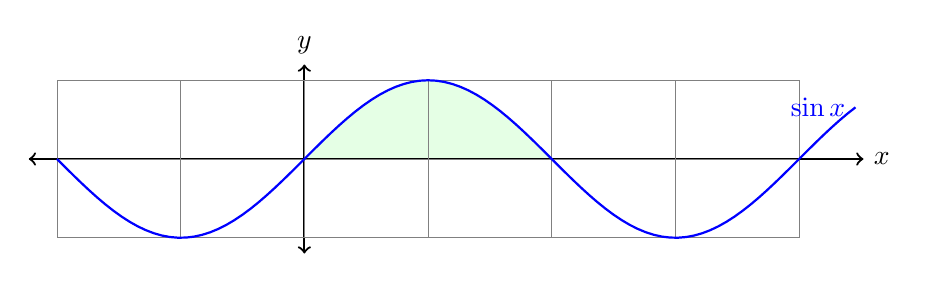
\begin{tikzpicture}

\filldraw[draw=none,fill=green!10]
plot [domain=0:pi] (\x,{sin(\x r)})
-- cycle;

\draw[thick,<->] (-3.5,0)--(7.1,0) node[right] {$x$};
\draw[thick,<->] (0,-1.2)--(0,1.2) node[above] {$y$}; 
\draw[color=gray,help lines, xstep=pi/2] (-pi,-1) grid (2*pi,1);

\draw [domain=-pi:7, blue,samples=100, thick] plot (\x,{sin(\x r)}) node[left] {$\sin x$}; 
\end{tikzpicture}
\end{adjustbox}
\end{figure}


\begin{figure}[H]
\centering
\begin{adjustbox} {width=0.4\textwidth}
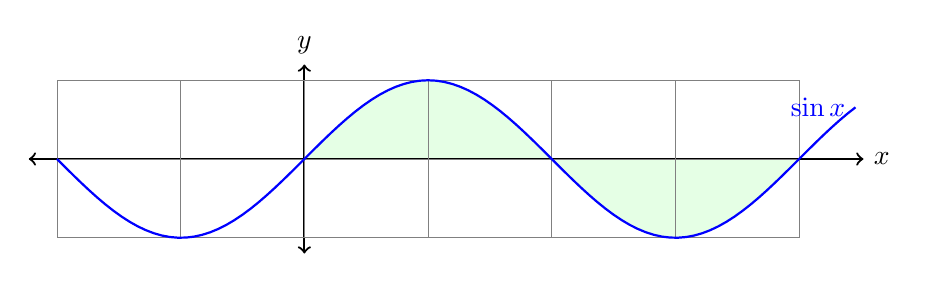
\begin{tikzpicture}

\filldraw[draw=none,fill=green!10]
plot [domain=0:2*pi] (\x,{sin(\x r)})
-- cycle;

\draw[thick,<->] (-3.5,0)--(7.1,0) node[right] {$x$};
\draw[thick,<->] (0,-1.2)--(0,1.2) node[above] {$y$}; 
\draw[color=gray,help lines, xstep=pi/2] (-pi,-1) grid (2*pi,1);

\draw [domain=-pi:7, blue,samples=100, thick] plot (\x,{sin(\x r)}) node[left] {$\sin x$}; 
\end{tikzpicture}
\end{adjustbox}
\end{figure}

\begin{figure}[H]
\centering
\begin{adjustbox} {width=0.4\textwidth}
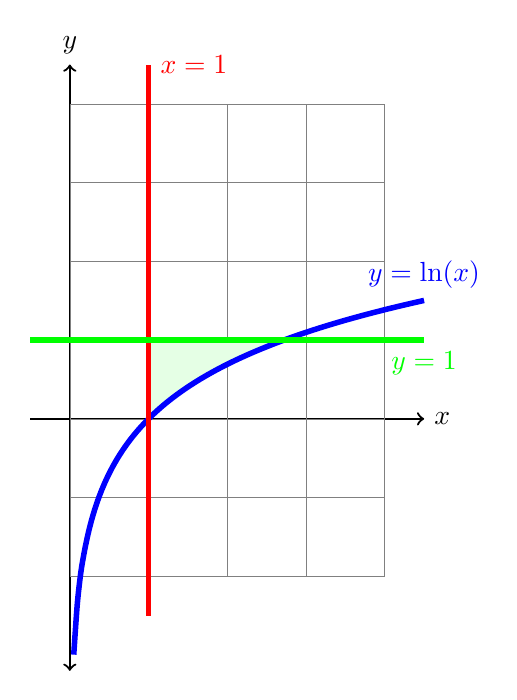
\begin{tikzpicture}
\draw[thick,->] (-0.5,0)--(4.5,0) node[right] {$x$};
\draw[thick,<->] (0,-3.2)--(0,4.5) node[above] {$y$}; 
\draw[color=gray,help lines] (0,-2) grid (4,4);

\filldraw[draw=none,fill=green!10] plot[smooth,domain=1:e](\x,{ln((\x))}) -- (1,1) -- cycle;  

\draw [blue,line width=2.pt,smooth,samples=100,domain=0.05:4.5] plot(\x,{ln((\x))}) node[above] {$y=\ln(x)$};

\draw[red, line width=2, domain=-2.5:4.5]  plot (1, {\x}) node[right] {$x=1$};

\draw[green, line width=2, domain=-0.5:4.5]  plot (\x, {1}) node[below] {$y=1$};
\end{tikzpicture}
\end{adjustbox}
\end{figure}

\begin{figure}[H] 
\centering 
\begin{adjustbox}{width=0.4\textwidth} 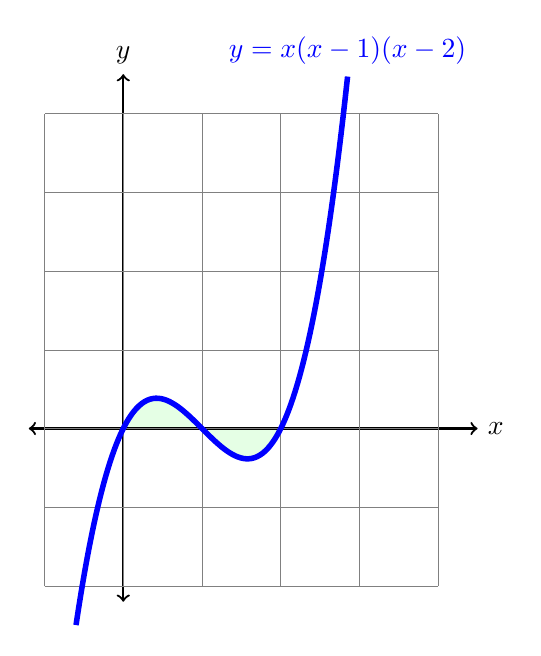
\begin{tikzpicture}

\filldraw[draw=none,fill=green!10] plot[smooth,domain=0:2](\x,{\x*(\x-1)*(\x-2)}) -- cycle;

\draw[thick,<->] (-1.2,0)--(4.5,0) node[right] {$x$};
\draw[thick,<->] (0,-2.2)--(0,4.5) node[above] {$y$};  

\draw[color=gray,help lines] (-1,-2) grid (4,4);

\draw [blue,line width=2.pt,smooth,samples=100,domain=-0.6:2.85] plot(\x,{\x*(\x-1)*(\x-2)}) node[above] {$y=x(x-1)(x-2)$};
\end{tikzpicture} 
\end{adjustbox}
\end{figure}


\begin{figure}[H] 
\centering 
\begin{adjustbox}{width=0.4\textwidth} 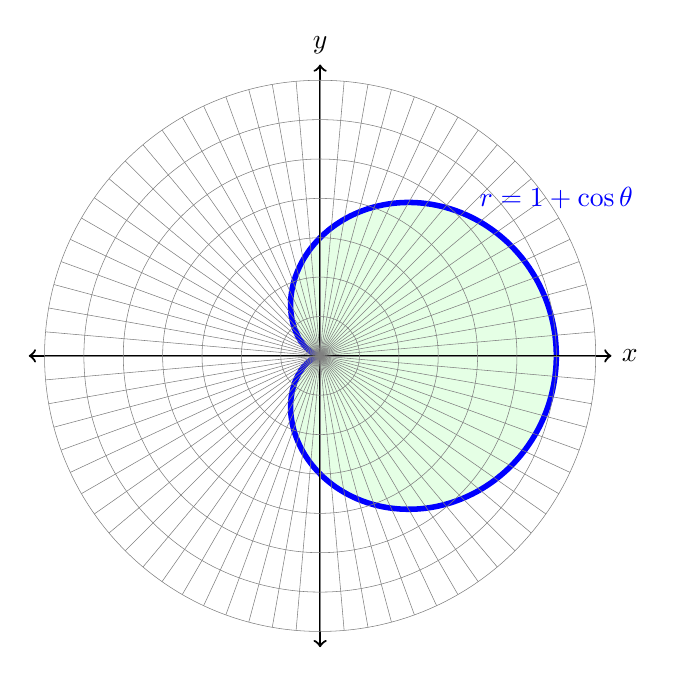
\begin{tikzpicture}

\filldraw[draw=blue,line width=2.pt,fill=green!10,domain=0:3*pi,scale=1.5,samples=500] plot ({deg(\x)}:{1+cos(\x r)});


\draw[thick,<->] (-3.7,0)--(3.7,0) node[right] {$x$};
\draw[thick,<->] (0,-3.7)--(0,3.7) node[above] {$y$};  

\foreach \x in {0,0.5,...,3.5}
\draw[help lines] (0,0) circle(\x);

\foreach \y in {0,5,...,360}
\draw[help lines] (0,0) -- (\y:3.5);

\node[blue] at (3,2) {$r=1+\cos \theta$};
\end{tikzpicture} 
\end{adjustbox}
\end{figure}

\begin{figure}[H] 
\centering 
\begin{adjustbox}{width=0.4\textwidth} 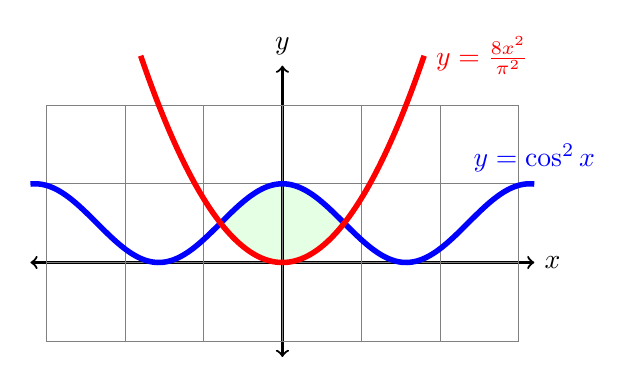
\begin{tikzpicture}

\filldraw[draw=none,fill=green!10] plot[smooth,domain=-pi/4:pi/4] (\x,{8*\x*\x/pi^2}) -- plot[smooth,domain=-pi/4:pi/4] (\x,{(cos(\x r))^2});

\draw[thick,<->] (-3.2,0)--(3.2,0) node[right] {$x$};
\draw[thick,<->] (0,-1.2)--(0,2.5) node[above] {$y$};  

\draw[color=gray,help lines] (-3,-1) grid (3,2);

\draw [blue,line width=2.pt,smooth,samples=100,domain=-3.2:3.2] plot(\x,{(cos(\x r))^2}) node[above] {$y=\cos^2 x$};

\draw [red,line width=2.pt,smooth,samples=100,domain=-1.8:1.8] plot(\x,{8*\x*\x/pi^2}) node[right] {$y=\frac{8x^2}{\pi^2}$};
\end{tikzpicture} 
\end{adjustbox}
\end{figure}

\begin{figure}[H] 
\centering 
\begin{adjustbox}{width=0.4\textwidth} 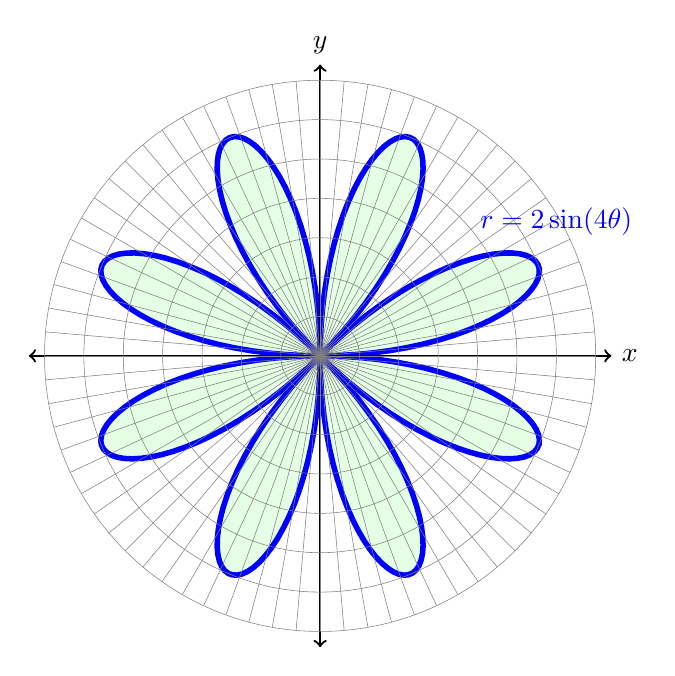
\begin{tikzpicture}

\filldraw[draw=blue,line width=2.pt,fill=green!10,domain=0:3*pi,scale=1.5,samples=500] plot ({deg(\x)}:{2*sin(4*\x r)});

\draw[thick,<->] (-3.7,0)--(3.7,0) node[right] {$x$};
\draw[thick,<->] (0,-3.7)--(0,3.7) node[above] {$y$};  

\foreach \x in {0,0.5,...,3.5}
\draw[help lines] (0,0) circle(\x);

\foreach \y in {0,5,...,360}
\draw[help lines] (0,0) -- (\y:3.5);

\node[blue] at (3,1.7) {$r=2\sin(4\theta)$};
\end{tikzpicture} 
\end{adjustbox}
\end{figure}

\begin{figure}[H] 
\centering 
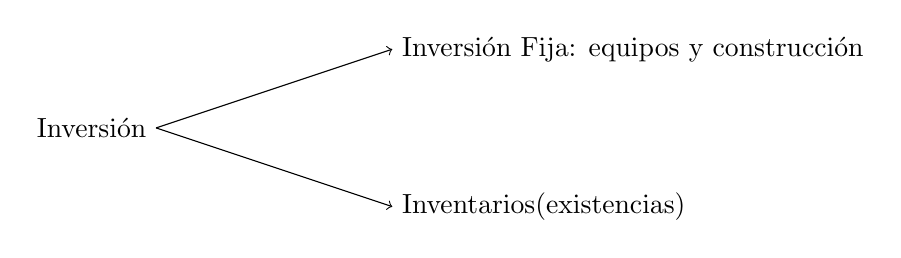
\begin{tikzpicture}
\node[left] at (0,0) {Inversión};
\node[right] at (3,1) {{Inversión Fija: equipos y construcción}}; 
\node[right] at (3,-1) {Inventarios(existencias)}; 
\draw[->] (0,0) -- (3,1);
\draw[->] (0,0) -- (3,-1);
\end{tikzpicture} 
\end{figure}

\begin{figure}[H] 
\centering 
\begin{adjustbox}{width=0.9\columnwidth}
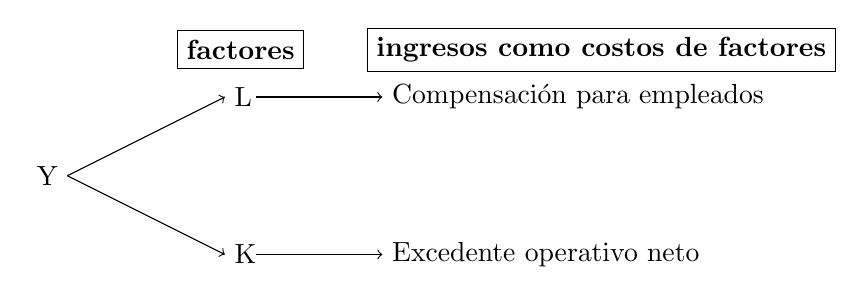
\begin{tikzpicture}
\node[left] at (0,0) {Y};

\node[draw] at (2.2,1.6) {\textbf{factores}};
\node[right] at (2,1) {L}; 
\node[right] at (2,-1) {K};


\node[draw, right] at (3.8,1.6) {\textbf{ingresos como costos de factores}};
\node[right] at (4,1) {Compensación para empleados};
\node[right] at (4,-1) {Excedente operativo neto};

\draw[->] (0,0) -- (2,1);
\draw[->] (0,0) -- (2,-1);
\draw[->] (2.4,1) -- (4,1);
\draw[->] (2.4,-1) -- (4,-1);
\end{tikzpicture}
\end{adjustbox}
\end{figure}

\end{document}

